\section{Desarrollo de Aplicación en Android}

\par 
El desarrollo de la aplicación en android no requiere de un software especializado como es en el caso de iOS. Solamente es necesario una computadora con un sistema operativo: windows, mac osx o linux. El entorno de desarrollo que utilizaremos es Android Studio; ya que, es soportado oficialmente por Google y recibe actualizaciones habitualmente. Adicional no es indispensable mas si es recomendable utilizar un dispositivo de prueba con la versión de android para cual estaremos desarrollando. Android Studio cuenta con un emulador con capacidad de emular la mayoria de los dispositivos android en el mercado; sin embargo, dependiendo de que tan reciente sea el dispositivo a emular, de la misma manera utilizará mas recursos del computador.

\clearpage

\par \noindent
Recordemos que el objetivo de la aplicación es el siguiente: establecer una comunicación bluetooth con nuestro prototipo y dependiendo de los parametros asignados por el usuario final. Capturar las mediciones de temperatura respetando los parametros seleccionados por el usuario y guardando los resultados en una base de datos local para ser consultados después.

\par \noindent
Nuestra aplicación requiere esencialmente de 3 elementos que debemos desarrollar: 

\begin{itemize}
	\item La interfaz
	\item Los Servicios del segundo plano
	\item La base de datos
\end{itemize}

\par \noindent
Como es necesario primero diseñar la interfaz para poder insertar datos en nuestra aplicación empezaremos por ahí. Cabe a destacar que la compañia SIGCSA nos a dado el permiso de utilizar los logos y colores oficiales de la compañia para el desarrollo de la aplicación.

\subsection{Interfaz de la Aplicación}

\par
Al inicio de la aplicación mostraremos una animación con el logo y el eslogan de la compañía. El tiempo de duración de esta animación es de 2 segundos y se ejecutara siempre y cuando la aplicación no entre en el segundo plano del sistema operativo. La imagen de la animación es la siguiente:

\begin{figure}[H]
	\centering
	
\includegraphics[width=0.2\linewidth]{interfaz1.png}
	\caption{Animación de inicio de la aplicación; también conocido como "Splash Screen"}
\end{figure}

\par \noindent
Transcurridos los 2 segundos de la animación automáticamente es reemplazado por la actividad principal.  

\subsubsection{Actividad Principal}

\begin{figure}[H]
	\centering
	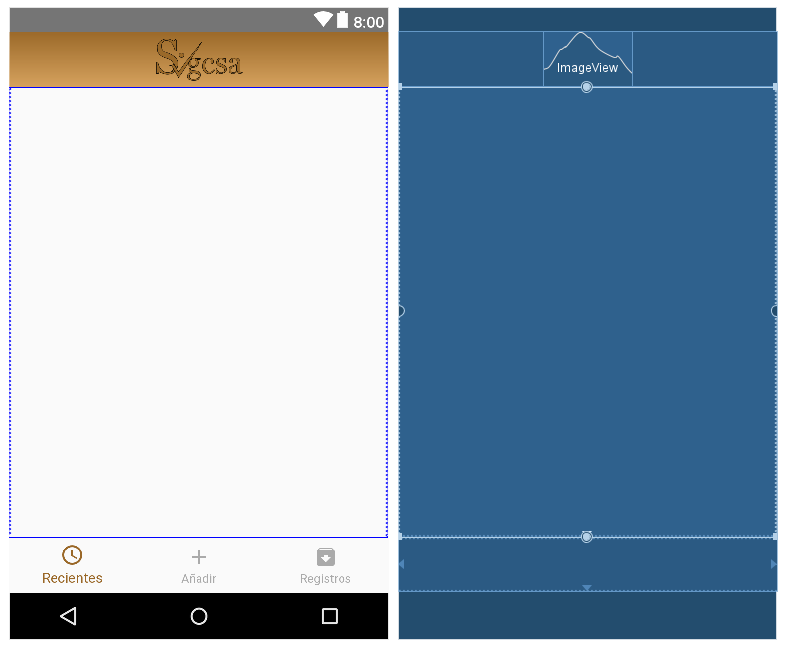
\includegraphics[width=0.8\linewidth]{interfaz2.png}
	\caption{Interfaz de la actividad principal}
\end{figure}

\par 
Pero ¿Qué es una actividad? y ¿Por qué es la actividad principal? Según la documentación oficial de Android una actividad se define como: un componente de aplicación que proporciona una pantalla con la que los usuarios pueden interactuar para hacer algo, como marcar el teléfono, tomar una foto, enviar un correo electrónico o ver un mapa. Una actividad puede iniciar otras actividades, incluidas actividades que viven en aplicaciones separadas.\cite{androidapp}

\par \noindent
Se ha llamado la actividad principal porque es donde el usuario final interactúa con el resto de los componentes de la aplicación tales como menús, actividades, fragmentos y servicios. 

\par \noindent
En la imagen 3.10 podemos apreciar los 3 componentes de la actividad principal. En la parte superior se encuentra el "toolbar", su objetivo es el de mostrar información relativa a la actividad donde se encuentra; por lo que, hemos elegido utilizar el logo de la compañía SIGCSA para enfatizar que es la actividad principal. 

\par \noindent
En la parte inferior nos encontramos con una tendencia en la navegación de la aplicación móviles hoy en día. En Android es llamado "BottomNavigationView", como su nombre lo indica es el encargado del manejo de las distintas fragmentos o subinterfaces utilizadas en una aplicación móvil. Es una cinta con el color de fondo de la aplicación en ella se encuentran botones que incluyen el texto y una pequeña imagen. Al seleccionar uno de estos botones la interfaz cambia con la excepción del "toolbar" y el "BottomNavigationView"; adicional el botón seleccionado incrementa ligeramente su tamaño y toma un color distinto al resto de los botones para indicar la interfaz activa en ese momento.

\par \noindent
El ultimo componente de la interfaz de la actividad principal no es visible para el usuario; sin embargo, se puede ver el borde azul en la imagen 3.10. Este componente es un "layout", en él es donde se pueden colocar otros componentes como botones, texto y más. Actúa realmente como un contenedor de componentes. En la actividad principal se encuentra vacío debido a que al iniciar la actividad debemos reemplazar este "layout" por una subinterfaz o fragmento. Por ende este componente es donde son expuestos los fragmentos seleccionados por el "BottonNavigationView" y nosotros hemos programado que el fragmento por defecto al iniciar esta actividad es el fragmento reciente.

\subsubsection{Fragmento Recientes}

\begin{figure}[H]
	\centering
	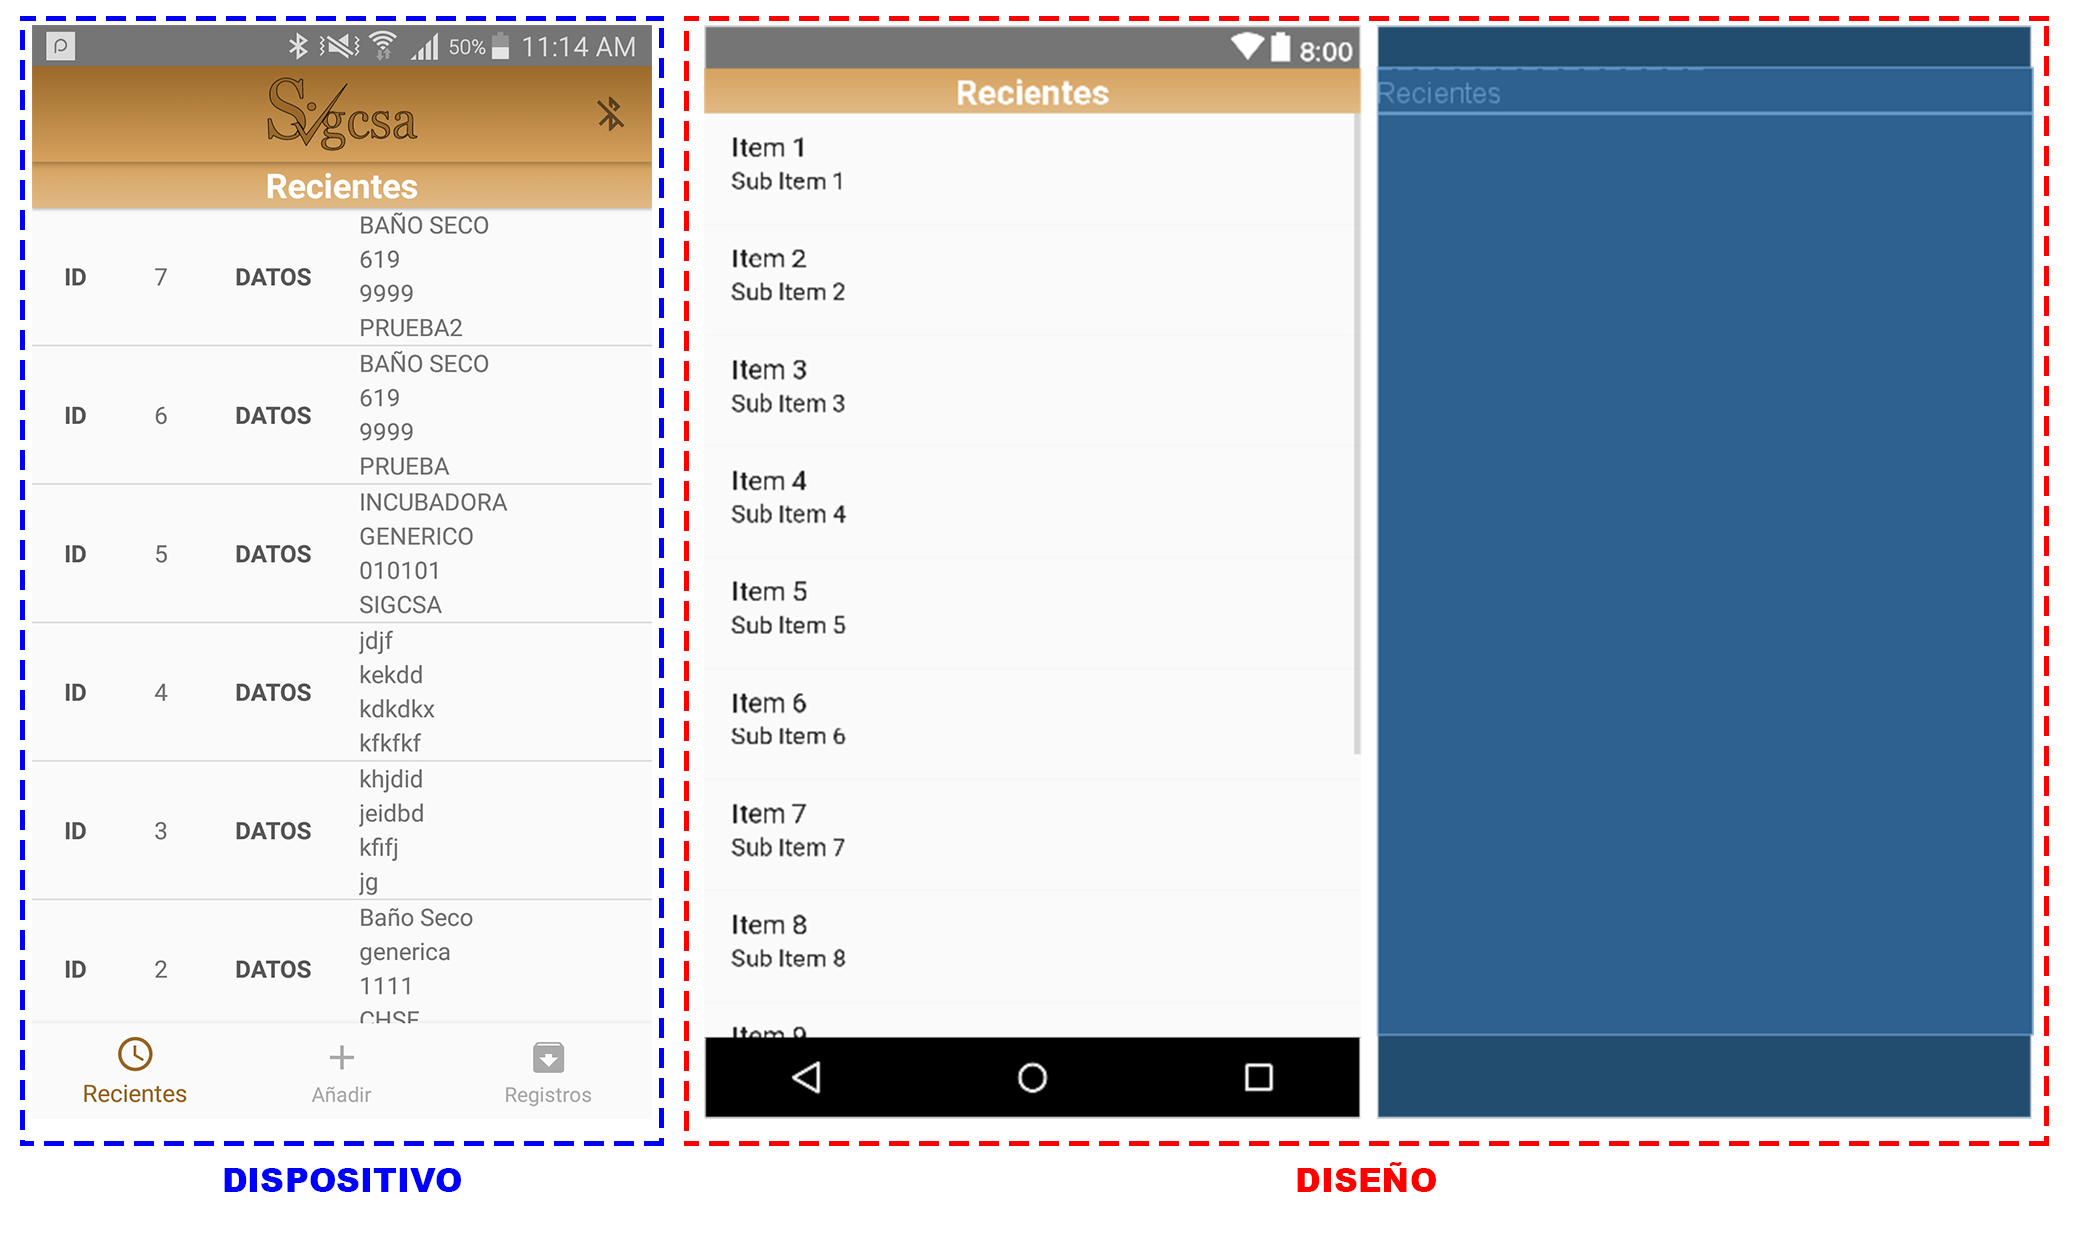
\includegraphics[width=\linewidth]{interfaz3.png}
	\caption{Interfaz del Fragmento Recientes en la aplicación y durante el diseño}
\end{figure}

\par \noindent
Al iniciar la aplicación, se inicia la actividad principal y el valor programado por defecto del "BottonNavegationView" es "Recientes"; por lo que, se procede a visualizar el fragmento reciente en la actividad principal. Un fragmento define una parte distinta del comportamiento de una actividad, incluida la interfaz de usuario asociada. Tiene su propio ciclo de vida que es similar al de la actividad y puede existir junto con otros fragmentos que están integrados en la actividad. Mientras se está ejecutando una actividad, puede agregar y eliminar fragmentos e incluir cada fragmento en una pila posterior administrada por la actividad, lo que permite al usuario navegar hacia atrás a través de los estados de los fragmentos, sin abandonar la actividad\cite{androidapp}. Está compuesto solamente por 3 componentes. 

\par \noindent
El componente principal es el "layout" que contiene los otros dos elementos que hacen la interfaz del usuario. Recordemos que es importante que los elementos de un fragmento se encuentren dentro de un "layout" ya que es más sencillo importar un layout a la actividad principal que todos los componentes por separado. El segundo componente es un "textview" su único objetivo es el de mostrar texto en la aplicación; sin embargo, puede ser utilizado para indicar al usuario partes de la interfaz. El "textview" despliega el texto "Recientes" y tiene un fondo similar al "toolbar" de la aplicación, esto es para brindar uniformidad en los colores de la aplicación. 

\par \noindent
El último elemento es un "ListView" es un componente especial porque podemos agregarle elementos de forma dinámica como una lista, podemos definirle la interfaz de sus elementos y cada elemento de la lista puede actuar como un botón para iniciar otra actividad. Es un elemento muy versátil e indispensable cuando trabajamos con bases de datos o cuando necesitamos ordenar información importante al usuario.

\begin{figure}[H]
	\centering
	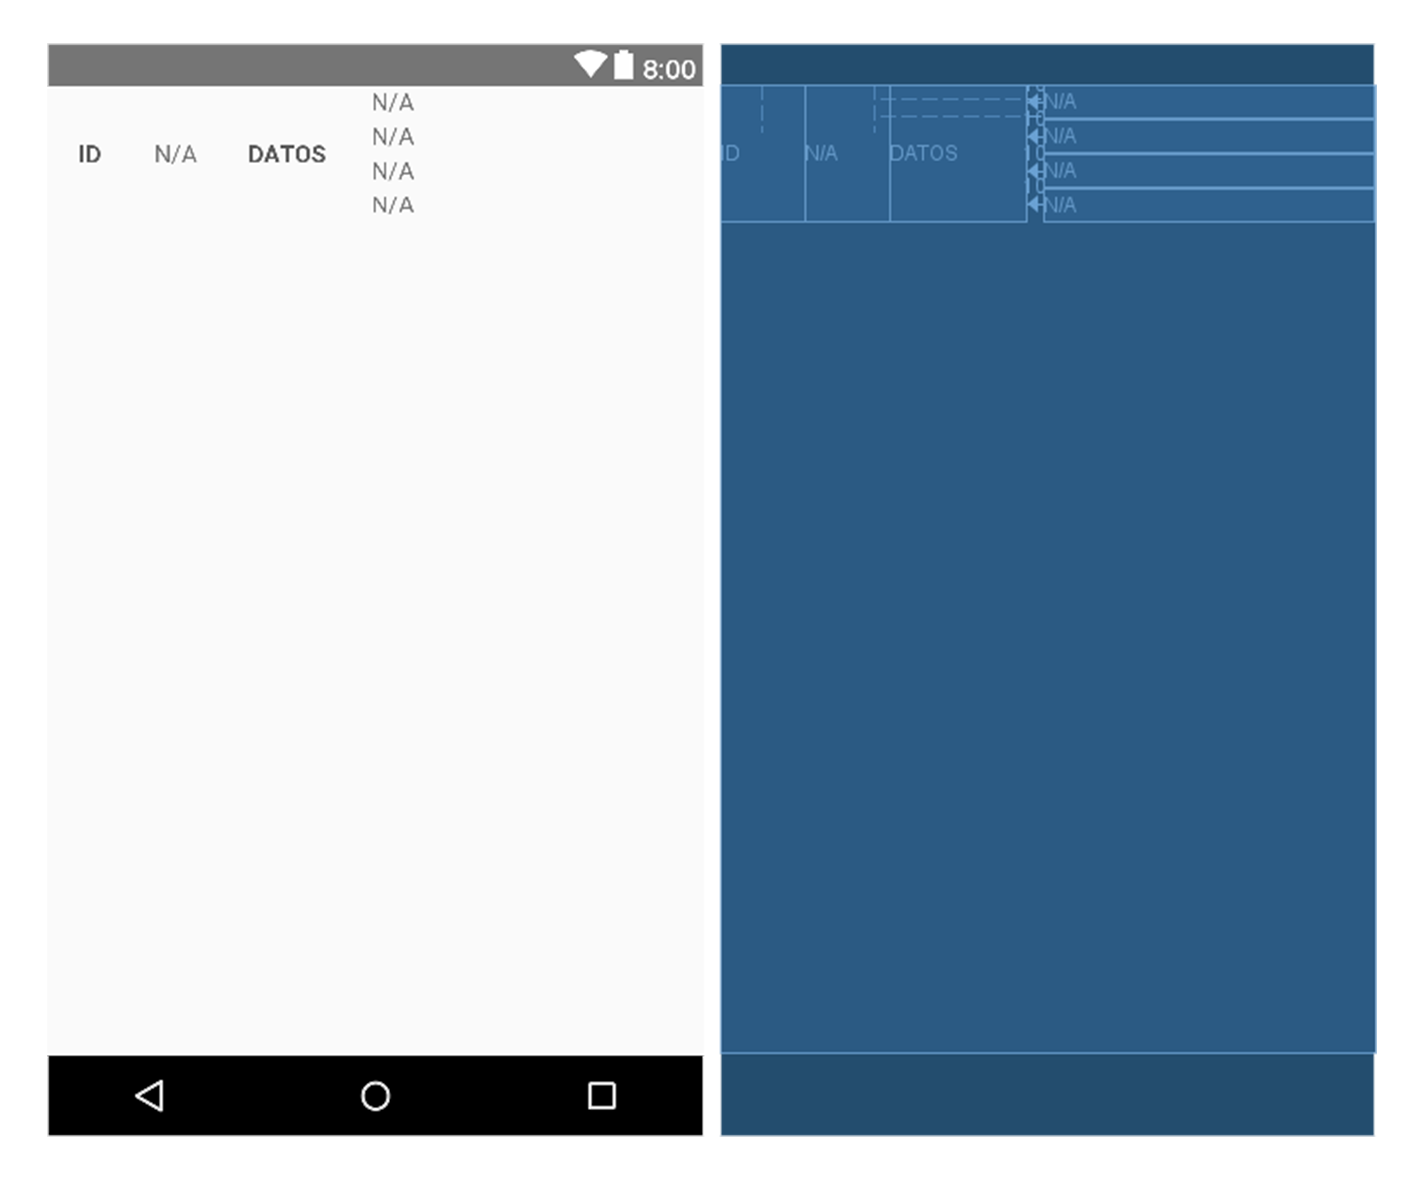
\includegraphics[width=0.5\linewidth]{interfaz4.png}
	\caption{Diseño de interfaz para "ListView" del fragmento recientes y registros}
\end{figure}

\par \noindent
El objetivo de este fragmento es el de mostrar las mediciones realizadas recientemente. Específicamente las ultimas 10 mediciones realizadas en nuestra aplicación. Mas adelante entraremos en detalle a lo que pasa cuando seleccionamos una de las mediciones mostradas en el "ListView". No obstante primero debemos saber cómo ingresamos datos al fragmento recientes. 

\subsubsection{Fragmento Añadir}

\begin{figure}[H]
	\centering
	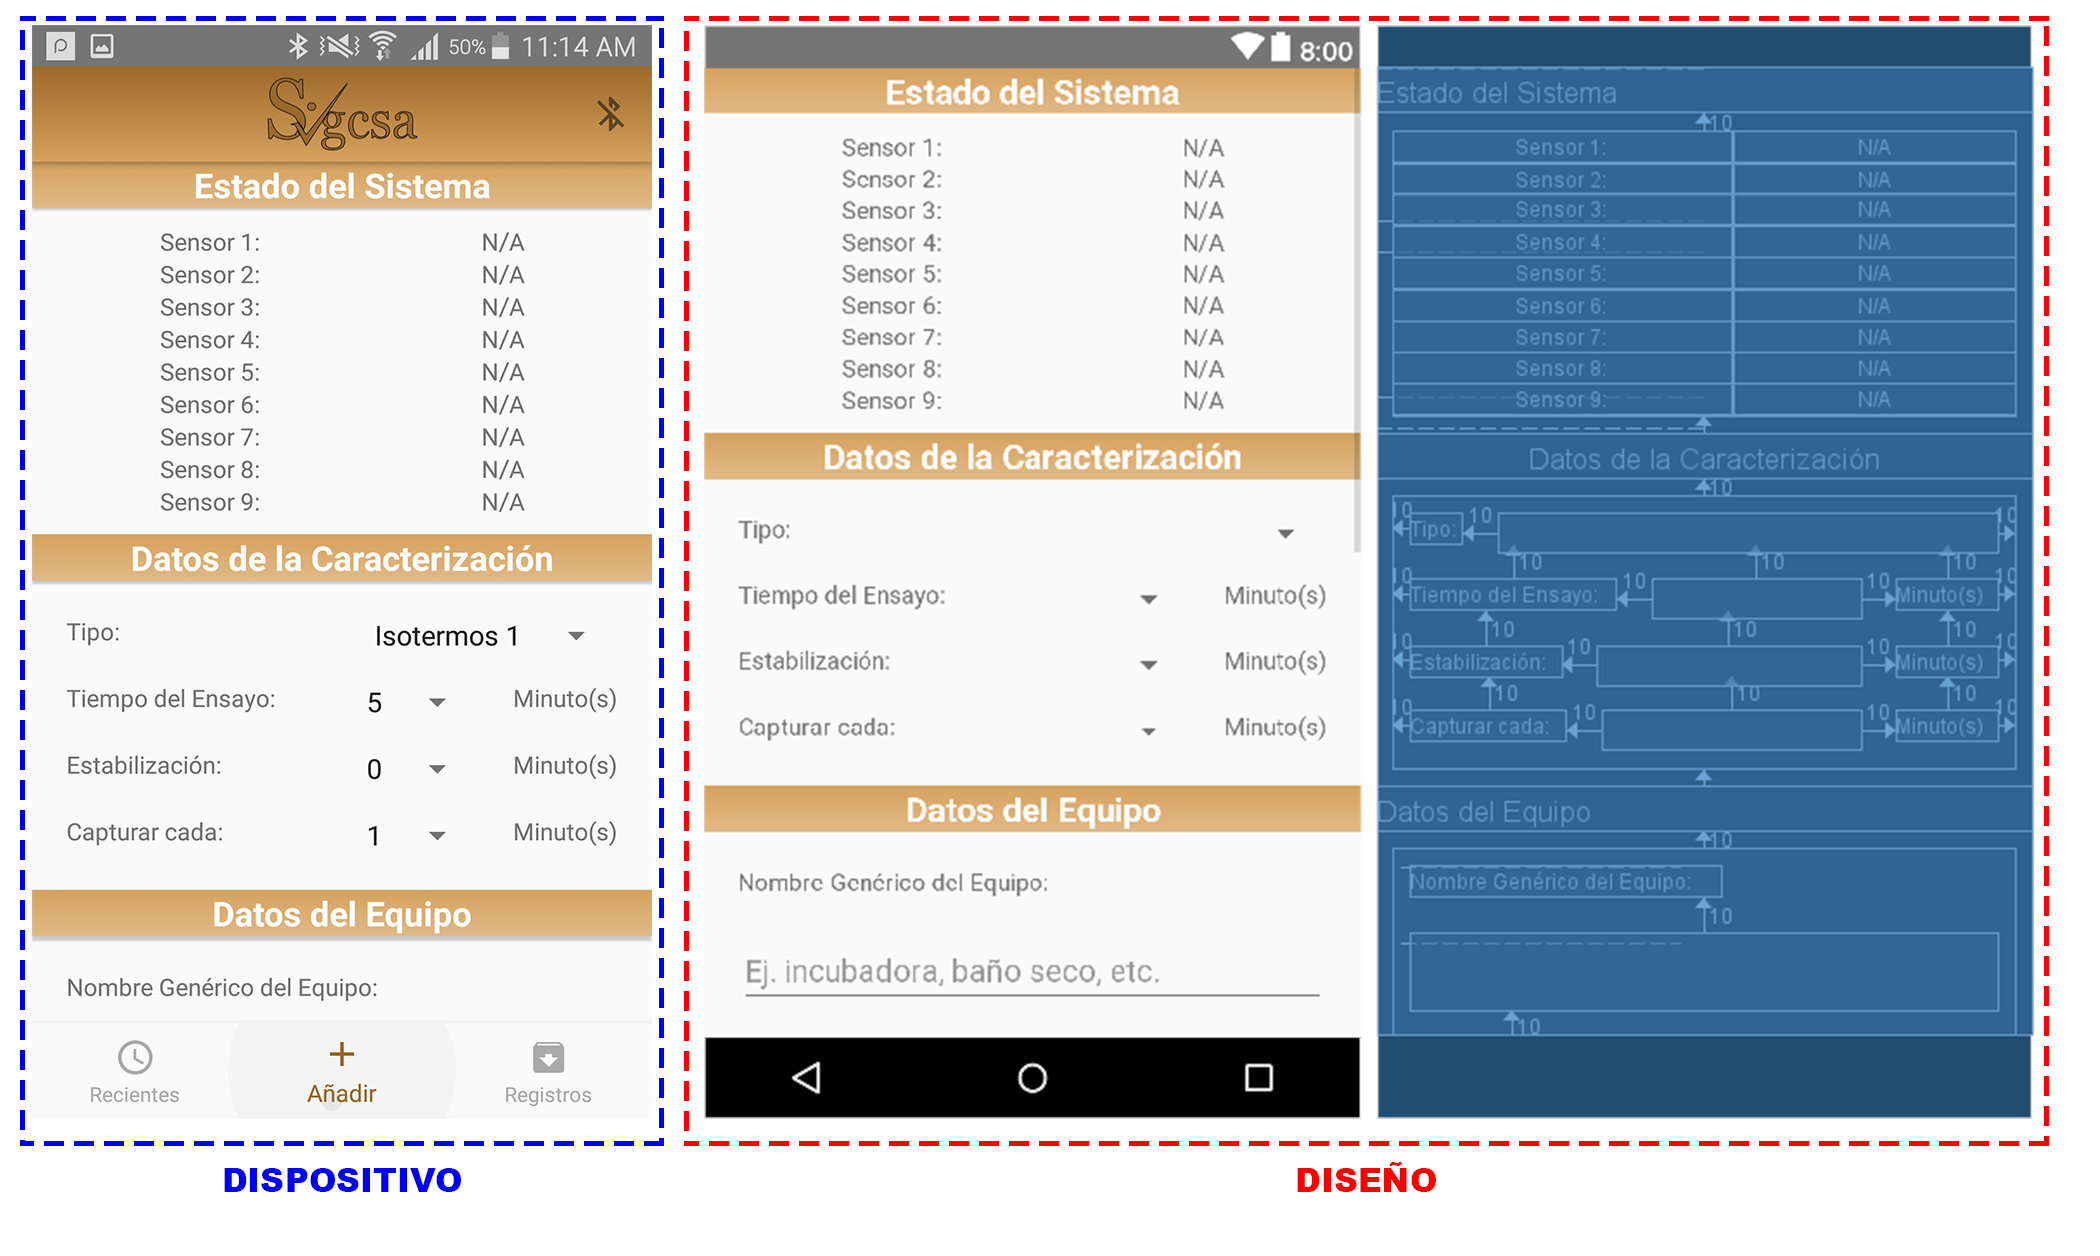
\includegraphics[width=\linewidth]{interfaz5.png}
	\caption{Interfaz del Fragmento Añadir en la aplicación y durante el diseño, parte 1}
\end{figure}

\par 
Fácilmente el fragmento añadir es la interfaz más compleja de este proyecto. El "Layout" utilizado para esta interfaz es un "ScrollView" el cual básicamente es un contenedor con características de desplazamiento vertical. El "ScrollView" es utilizado debido a que todos los elementos de la interfaz no caben en una pantalla promedio de un smartphone. Dentro del "ScrollView" encontramos un "Layout" específicamente un "RelativeLayout" el cual permite un manejo eficiente de los elementos que conforman la interfaz del usuario. 

\par \noindent
El fragmento añadir se divide en 3 secciones. Al inicio el "Estado del Sistema", seguido de “Datos de la Caracterización" y "Datos del Equipo". Estas secciones son dividas por un simple texto con fondo; con el objetivo de mantener la aplicación fluida al usuario.

\begin{figure}[H]
	\centering
	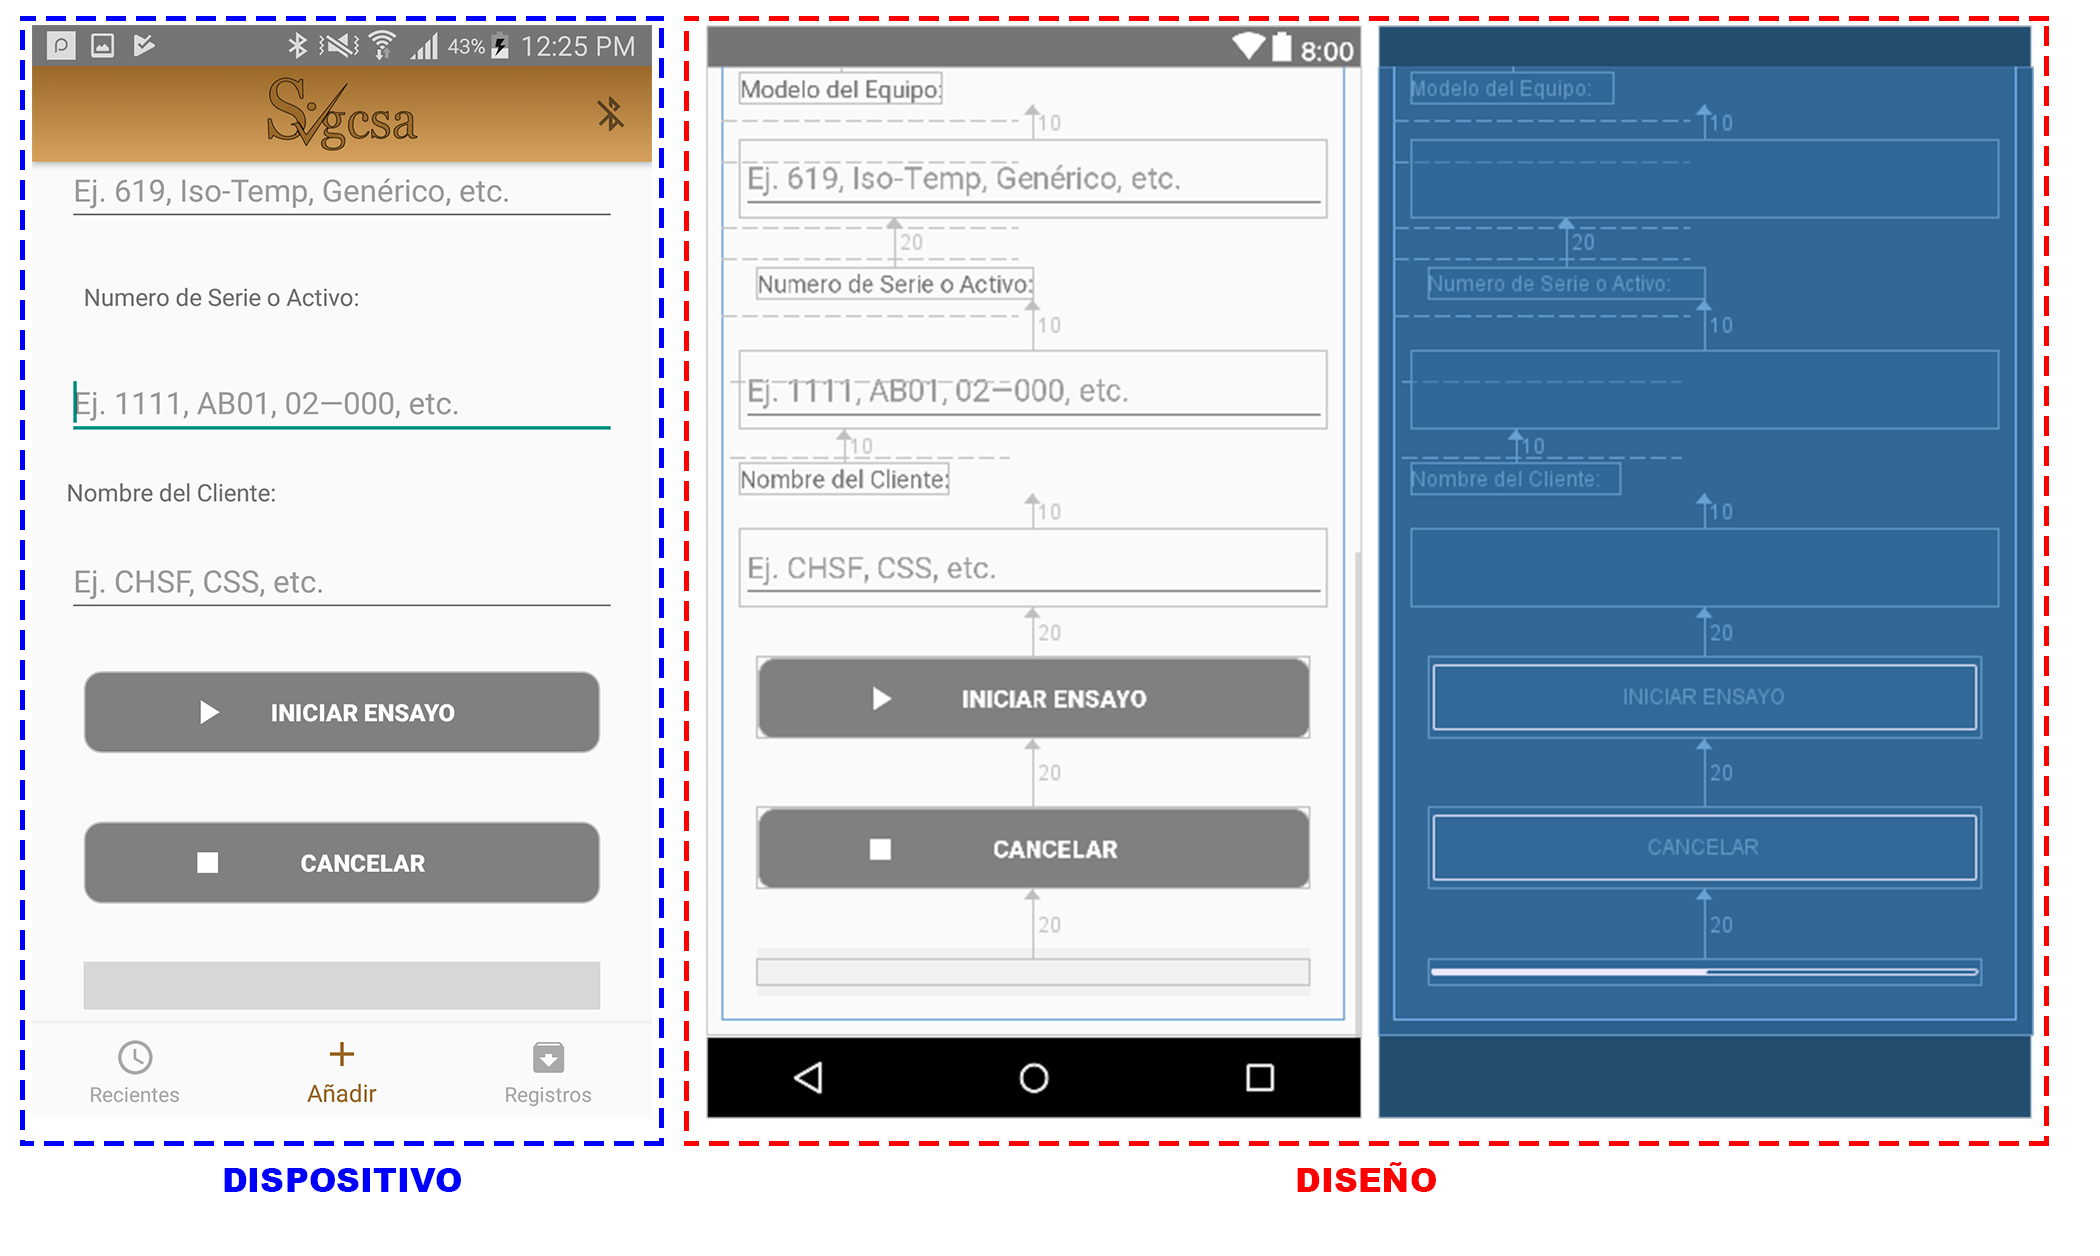
\includegraphics[width=\linewidth]{interfaz6.png}
	\caption{Interfaz del Fragmento Añadir en la aplicación y durante el diseño, parte 2}
\end{figure}

\par \noindent
La sección "Estado del Sistema" contiene los textos que visualizaran las temperaturas de los prototipos; ver imagen 3.13, una vez sea establecida la comunicación por bluetooth. A la izquierda es una guía del número de sonda o prototipo y a la derecha se encuentra el texto "N/A"; sin embargo, este valor cambiará a la temperatura actual obtenida por su respectivo prototipo y en caso tal de no recibir una lectura se mantendrá en el texto "N/A".

\par \noindent
La sección "Datos de la Caracterización" contiene los parámetros que definirá el usuario para determinar las características de la medición o ensayo. En la imagen 3.13 podemos observar que esta sección consta de 4 casillas donde el usuario puede elegir opciones predeterminas.

\par \noindent
En las opciones de tipo hay 3 opciones: Isotermos 1, Isotermos 2 y Calibración con Patrón. Según el capítulo 3 donde se analizaron los procesos a automatizar podemos notar que los medios Isotermos 1 necesitan de 9 termómetros; mientras que, Isotermos 2 de 4 termómetros. Al saber esto debemos tener una interfaz dinámica; la cual dependiendo del tipo de ensayo que se seleccione muestre únicamente la cantidad de prototipos que necesitaremos. 

\begin{figure}[H]
	\centering
	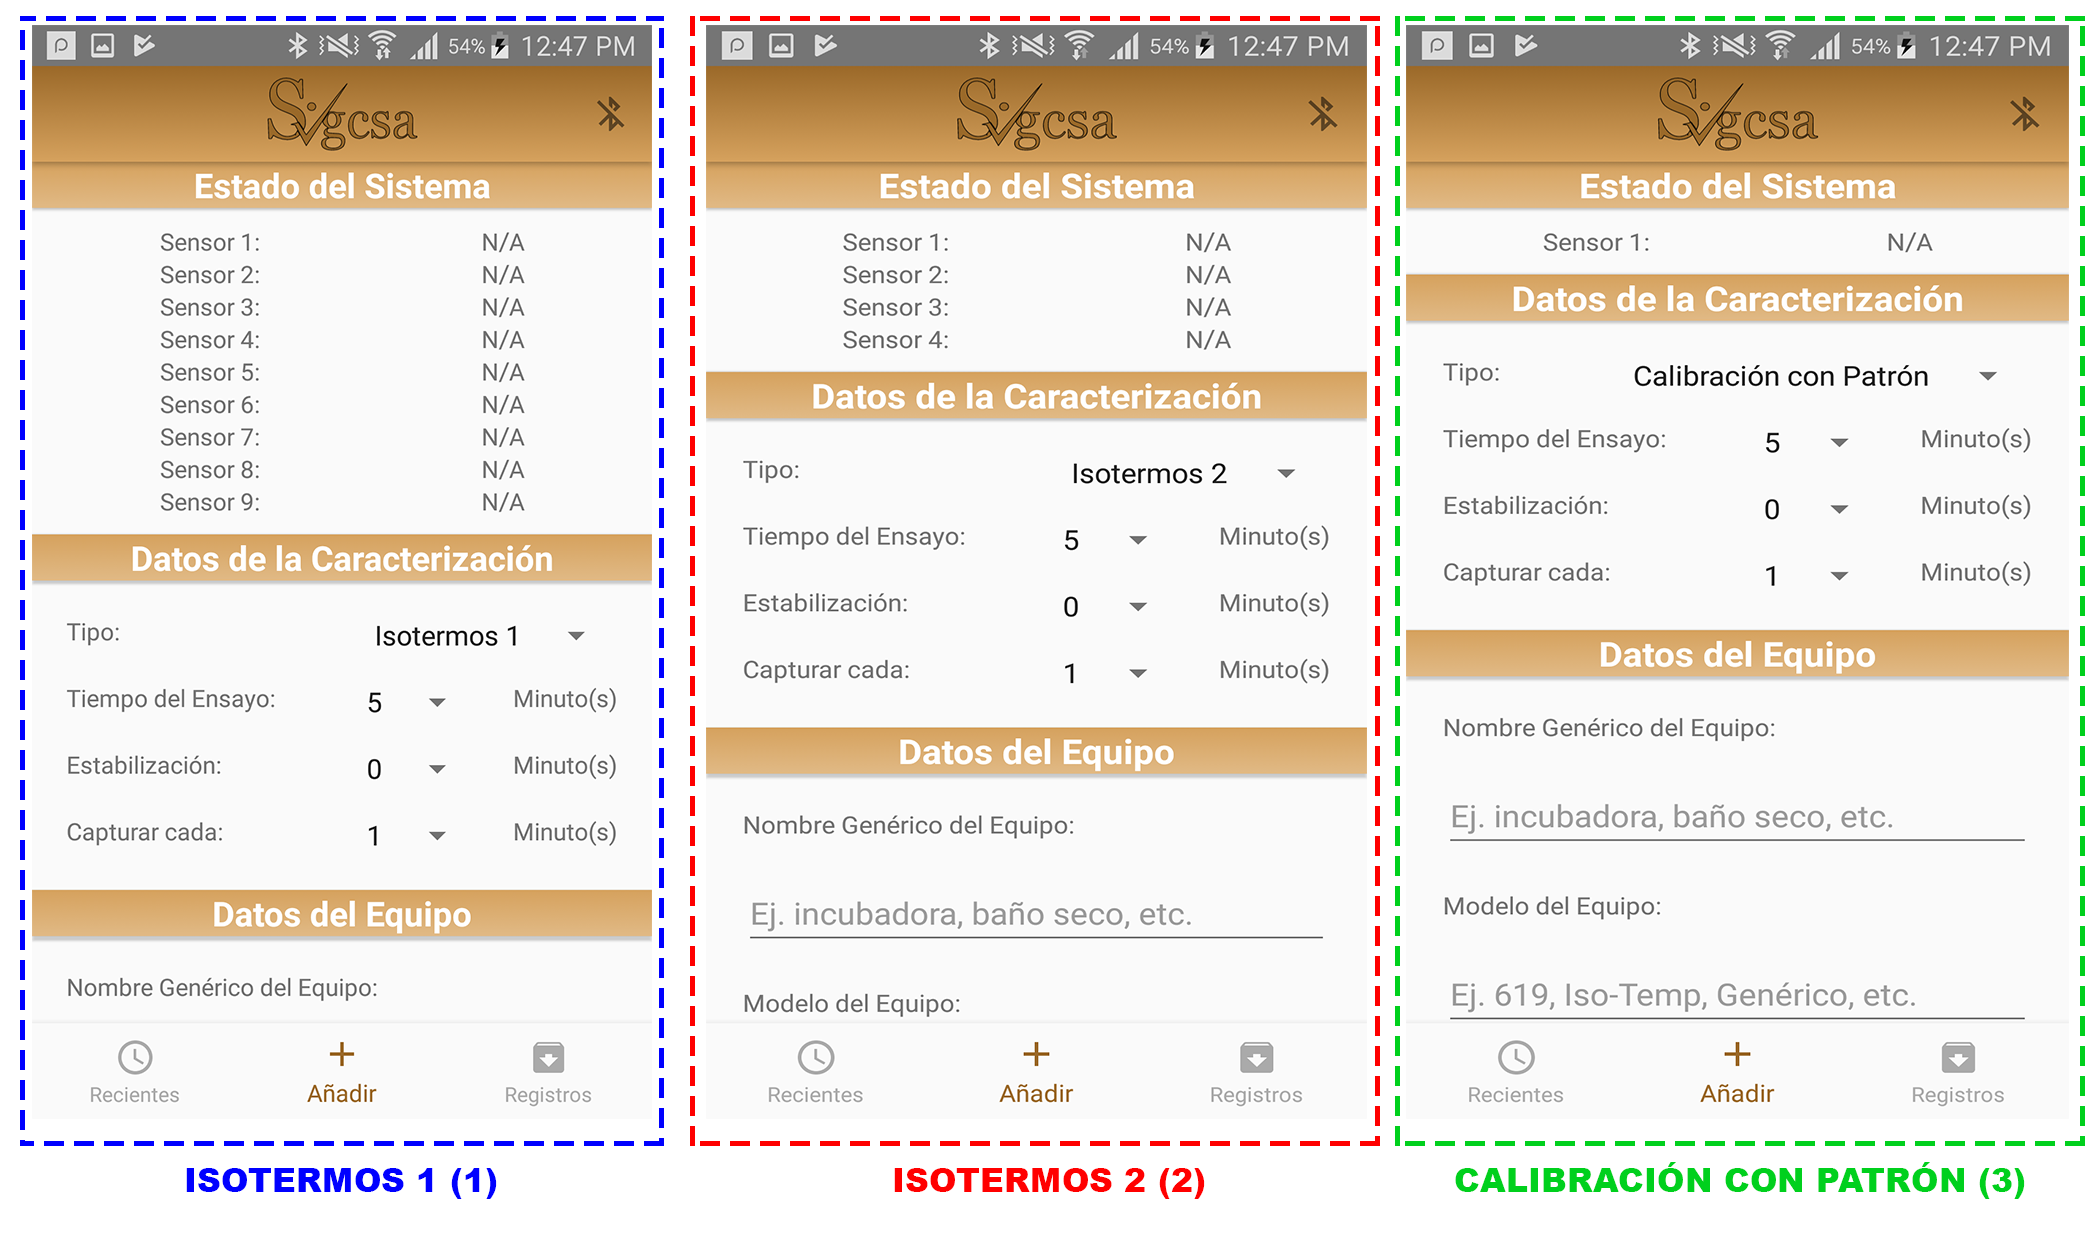
\includegraphics[width=\linewidth]{interfaz7.png}
	\caption{Dependiendo de la opción seleccionada, se ajustan los textos en la sección de "Estado del Sistema"}
\end{figure}

\par \noindent
Entre los otros parámetros de la sección "Datos de la Caracterización" se encuentran las casillas para "tiempo del ensayo" el cual determinará por cuanto tiempo se tomará las medidas de temperatura donde el mínimo son 5 minutos y el máximo es de 60 minutos o una hora. "Estabilización" es el tiempo previo que seleccionara el usuario final; en muchas ocasiones personal de campo esperan que la temperatura en un medio isotermo se estabilice antes de proceder a capturar las medidas. Por último "Capturar cada" se explica por sí misma, es el intervalo de tiempo en que se tomaran las medidas de temperatura.

\par \noindent
Como hemos mencionado esta interfaz contiene más componentes que las demás; por lo que, no todos los componentes de la interfaz pueden ser apreciados en una pantalla de un smartphone promedio. Se debe deslizar el fragmento para poder observar los componentes faltantes. Una vez realizado esto la interfaz quedara como la imagen 3.14. 

\par \noindent
La última sección "Datos del Equipo" cuenta con campos para ingresar información del equipo a realizar el ensayo de caracterización. Datos como nombre, modelo, serie y cliente. Adicional contamos con dos botones, uno para iniciar el servicio para el registro de mediciones y otro para cancelar dicho servicio. Por último hay un "progressbar" el cual se irá completando a medida que vaya avanzando el ensayo.

\subsubsection{Fragmento Registros}

\begin{figure}[H]
	\centering
	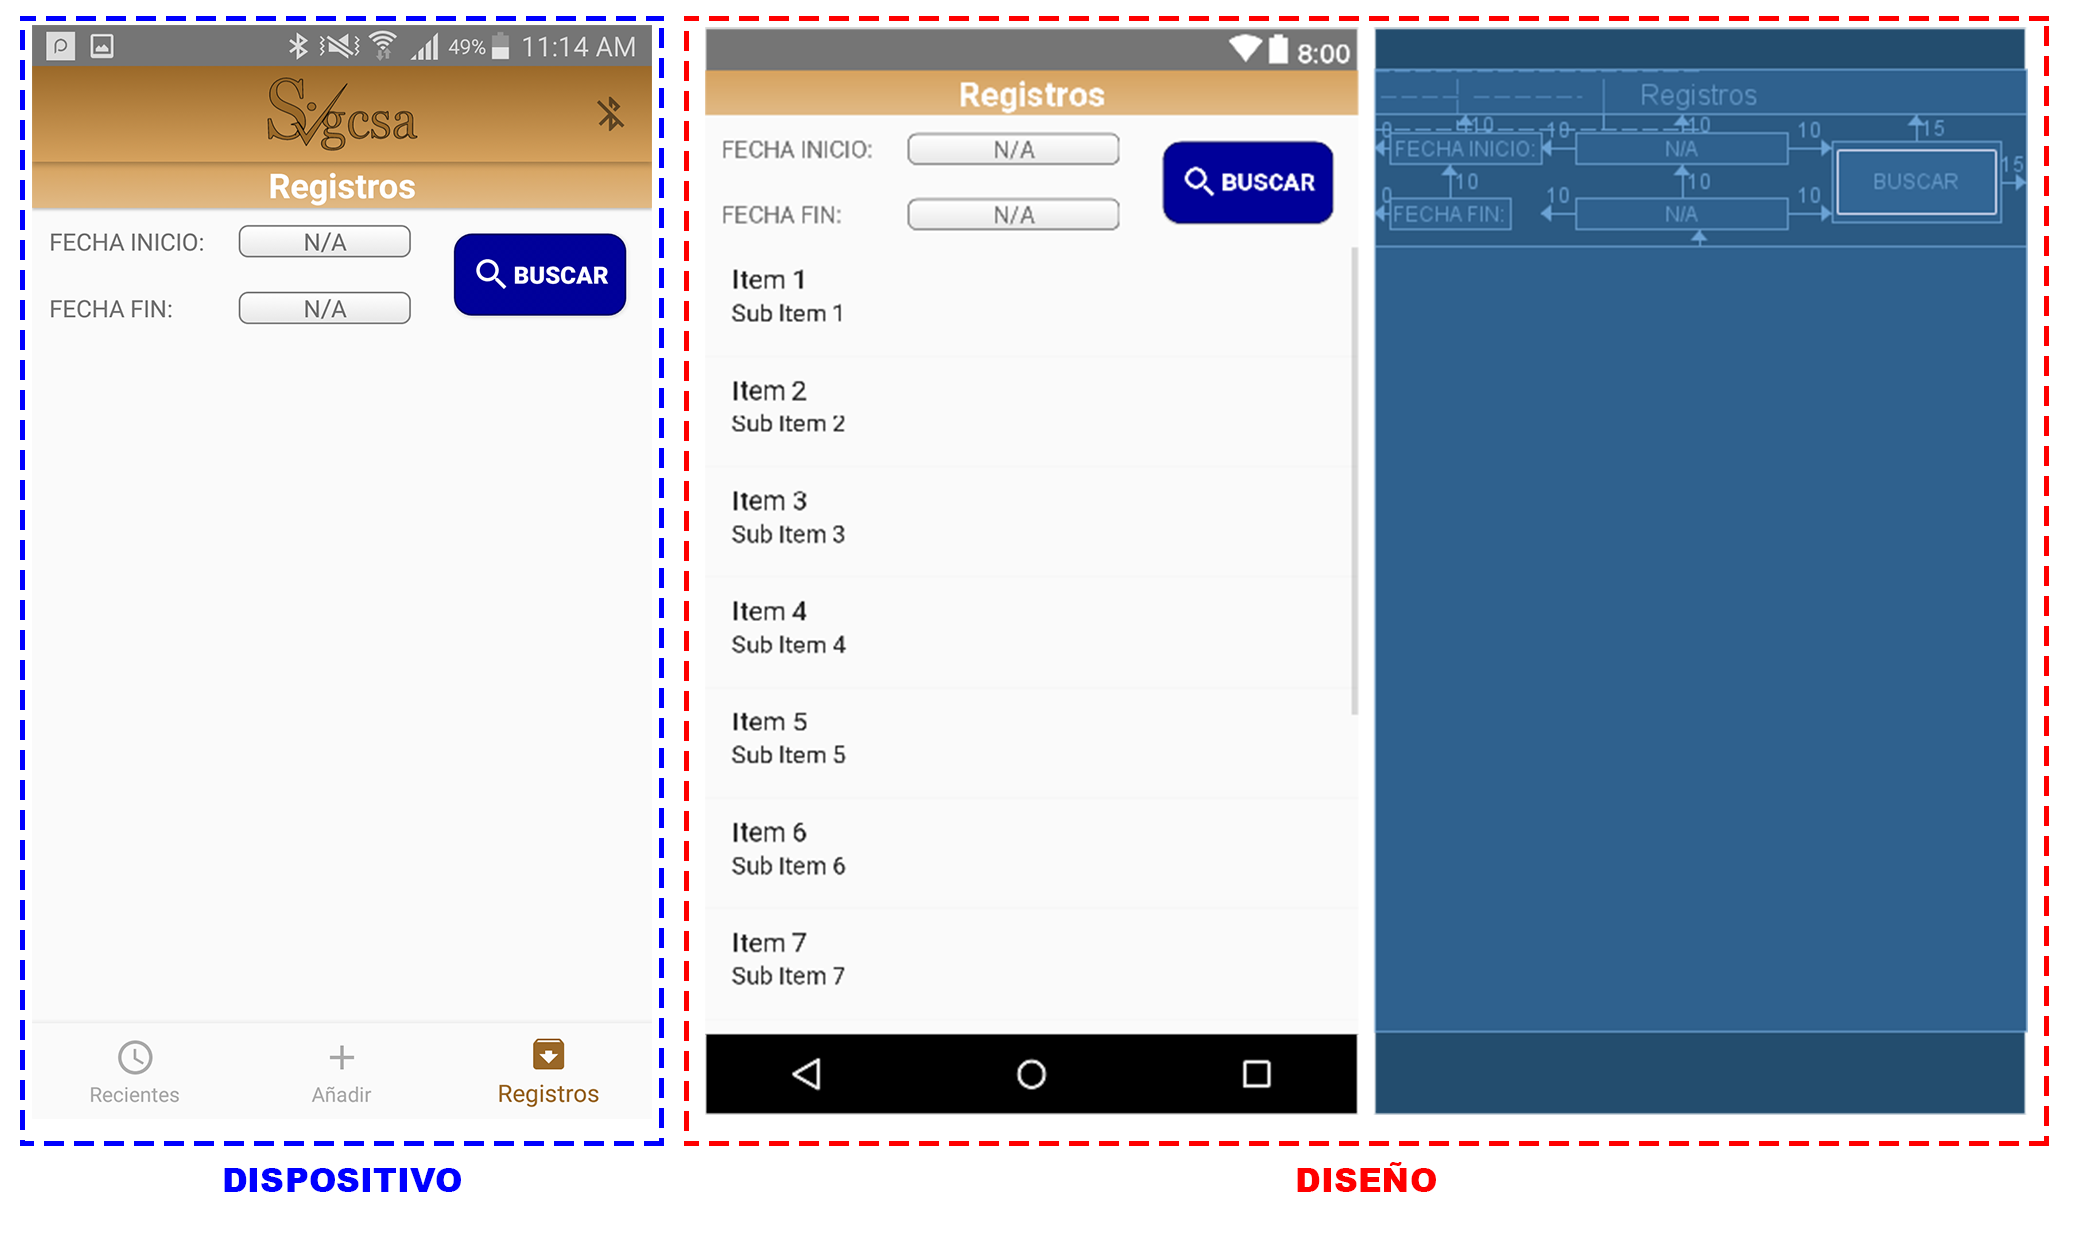
\includegraphics[width=\linewidth]{interfaz8.png}
	\caption{Interfaz y diseño del fragmento registros}
\end{figure}

\begin{figure}[H]
	\centering
	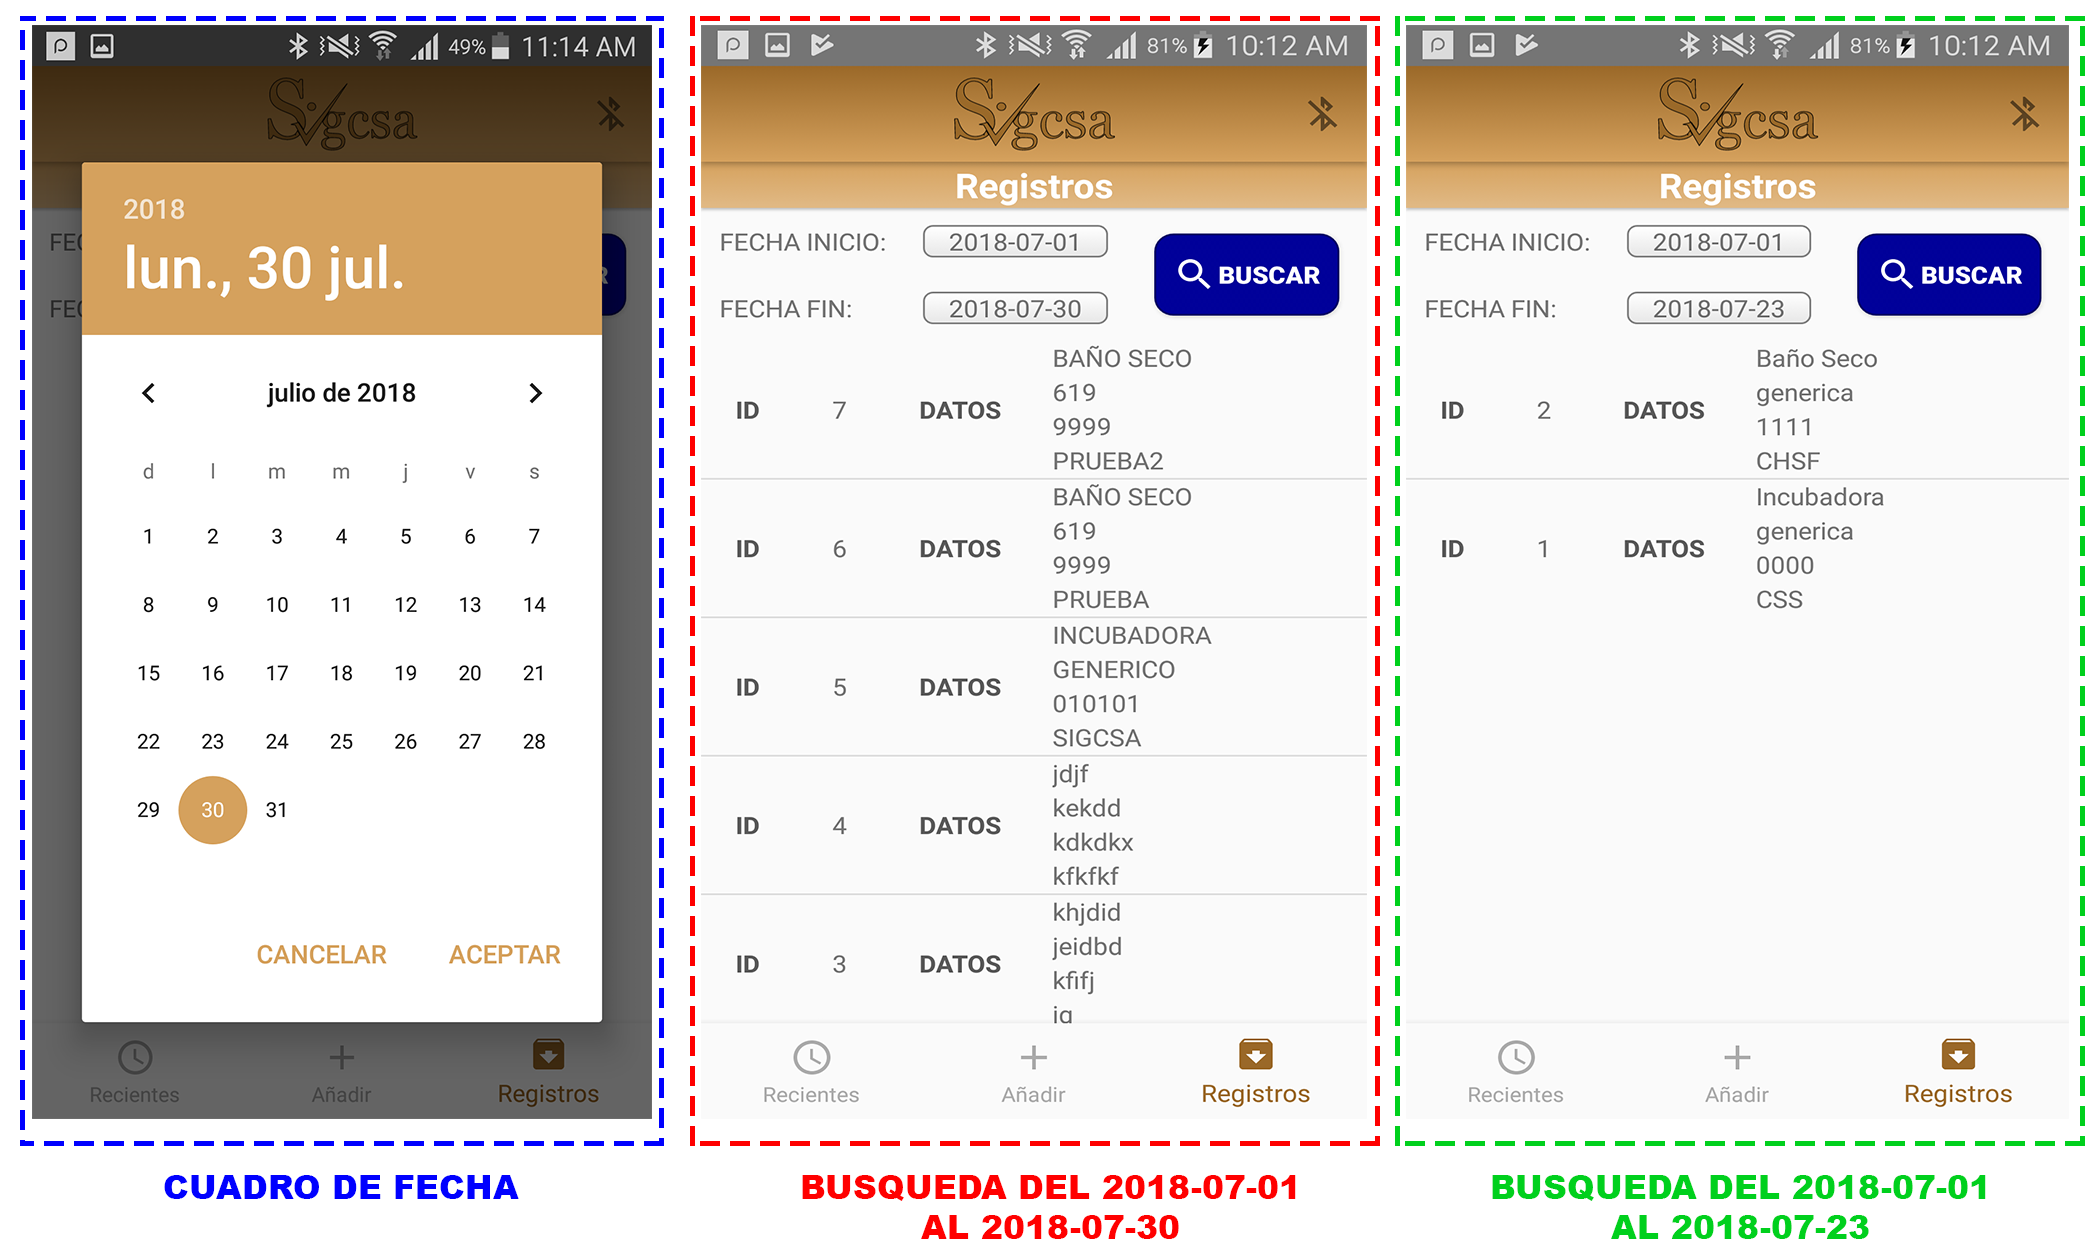
\includegraphics[width=\linewidth]{interfaz9.png}
	\caption{Cuadro de selección de fechas y resultados del fragmento registros dependiendo de la fecha}
\end{figure}

\par
El fragmento registros básicamente es una extensión del fragmento recientes, la única diferencia es que se puede definir las fechas de las mediciones (ensayos) que hemos realizado en nuestro smartphone. 

\par \noindent
Cuenta con textos que indican los botones para seleccionar fecha de inicio y fecha fin, al seleccionar uno de los botones se abre un cuadro con una interfaz amigable, ver imagen 3.17, para seleccionar la fecha deseada. Un botón de buscar el cual buscara las mediciones en la base de datos utilizando como parámetros las fechas seleccionadas. De encontrar resultados los despliega en un "ListView" del fragmento en cuestión. El comportamiento del "ListView" del fragmento registros es igual al del fragmento recientes.

\par \noindent
Estos tres fragmentos componen la actividad principal. Ya sabemos que es la primera que visualiza el usuario después de la animación inicial. Sabemos también que es donde se consulta la información de los ensayos realizados, estipulamos los parámetros de un ensayo, lo iniciamos o cancelamos y tenemos conocimiento en tiempo real de las temperaturas de los prototipos. Pero aún no sabemos dónde establecemos comunicación con nuestro prototipo. 

\subsubsection{Actividad Bluetooth}

\par 
La actividad bluetooth es la encargada de visualizar los equipos bluetooth disponibles. Establece comunicación con nuestro prototipo; ya que, es la encargada de llamar al servicio bluetooth de nuestra aplicación; la cual retroalimenta la actividad principal.

\par \noindent
En las imágenes 3.13, 3.14, 3.15, 3.16 y 3.17 podemos percatar en la esquina superior derecha de nuestra aplicación un pequeño icono de color gris con un símbolo de bluetooth. Si seleccionamos este icono llamamos a la actividad bluetooth. En ella podemos visualizar los dispositivos bluetooth disponibles. Está compuesta por un "toolbar" que con el texto "Conexiones Bluetooth" y botón para regresar a la actividad principal. Un texto con fondo que indica los dispositivos, un "ListView" en el cual se desplegaran los dispositivos disponibles. Por último un botón para actualizar el "ListView" en caso tal de querer establecer una conexión con nuevos dispositivos.

\begin{figure}[H]
	\centering
	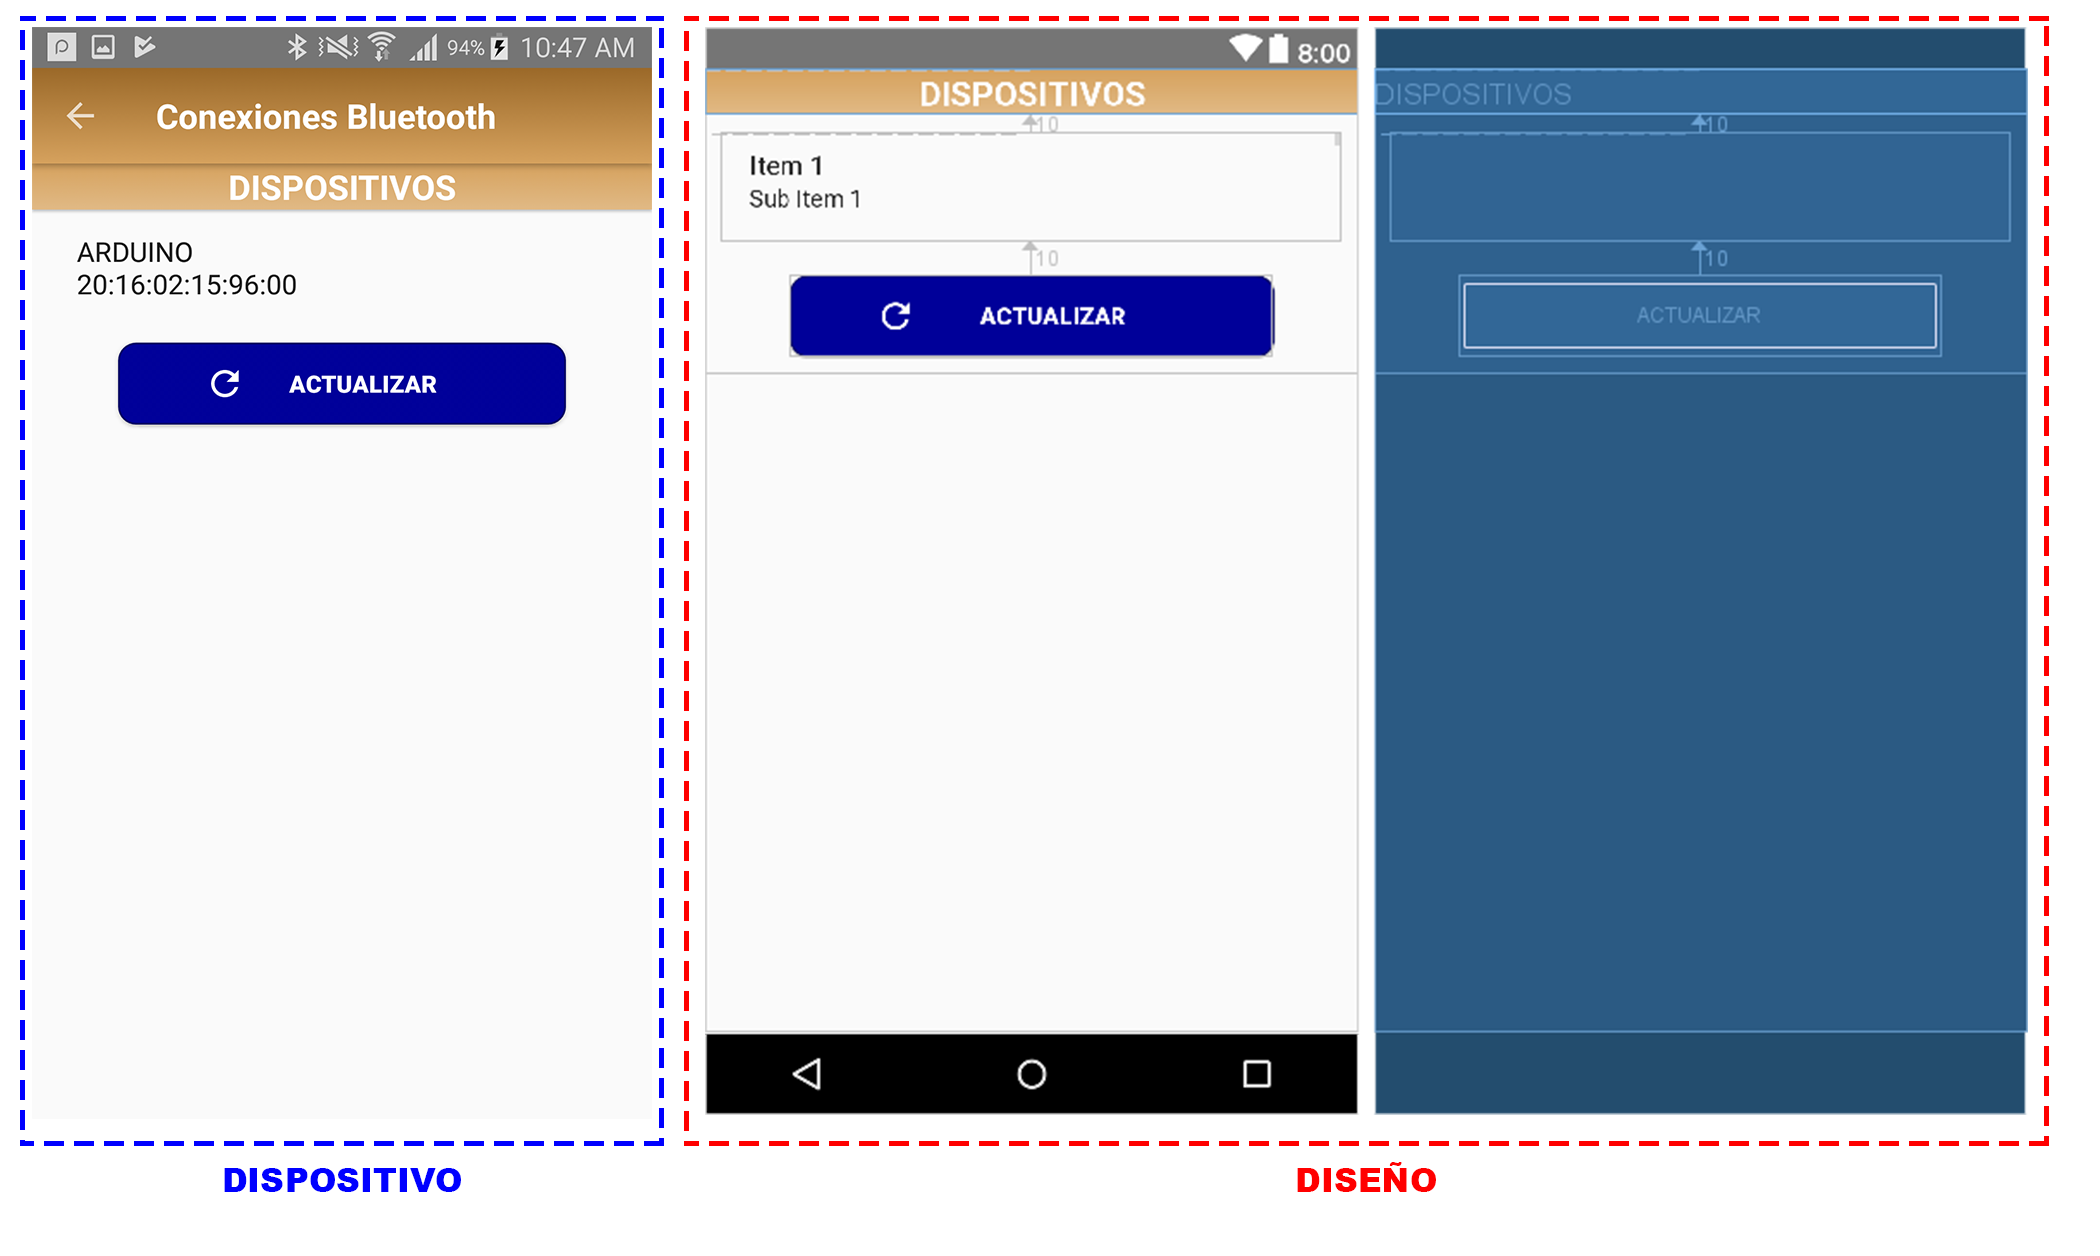
\includegraphics[width=\linewidth]{interfaz10.png}
	\caption{Interfaz y diseño de la actividad bluetooth}
\end{figure}

\par \noindent
La última tarea o función de que el usuario puede realizar en nuestra aplicación es el de consultar la información capturada. La actividad detalle es la encargada de demostrar la información capturada en los ensayos y las mediciones de los prototipos. Anteriormente en la sección de fragmento recientes y registros habíamos mencionado que el componente "ListView" tiene muchas características y que una de ellas era la de simular un botón por cada renglón de información desplegada al usuario. La actividad detalle es ejecutada al seleccionar una de la opción de los "ListView".

\subsubsection{Actividad Detalle}

\par 
En las imágenes 3.11 y 3.17 podemos observar los "ListView" donde se despliegan información de los ensayos realizados en la aplicación. Cada opción de ambas listas cuenta con información del ensayo que se encuentra en la base de datos de la aplicación. Al seleccionar una de las opciones se desplegará la actividad detalle. 

\par \noindent
En la Imagen 3.19 observamos que en la información y componentes de la interfaz se encuentran distribuida de manera similar al del fragmento añadir.

\begin{figure}[H]
	\centering
	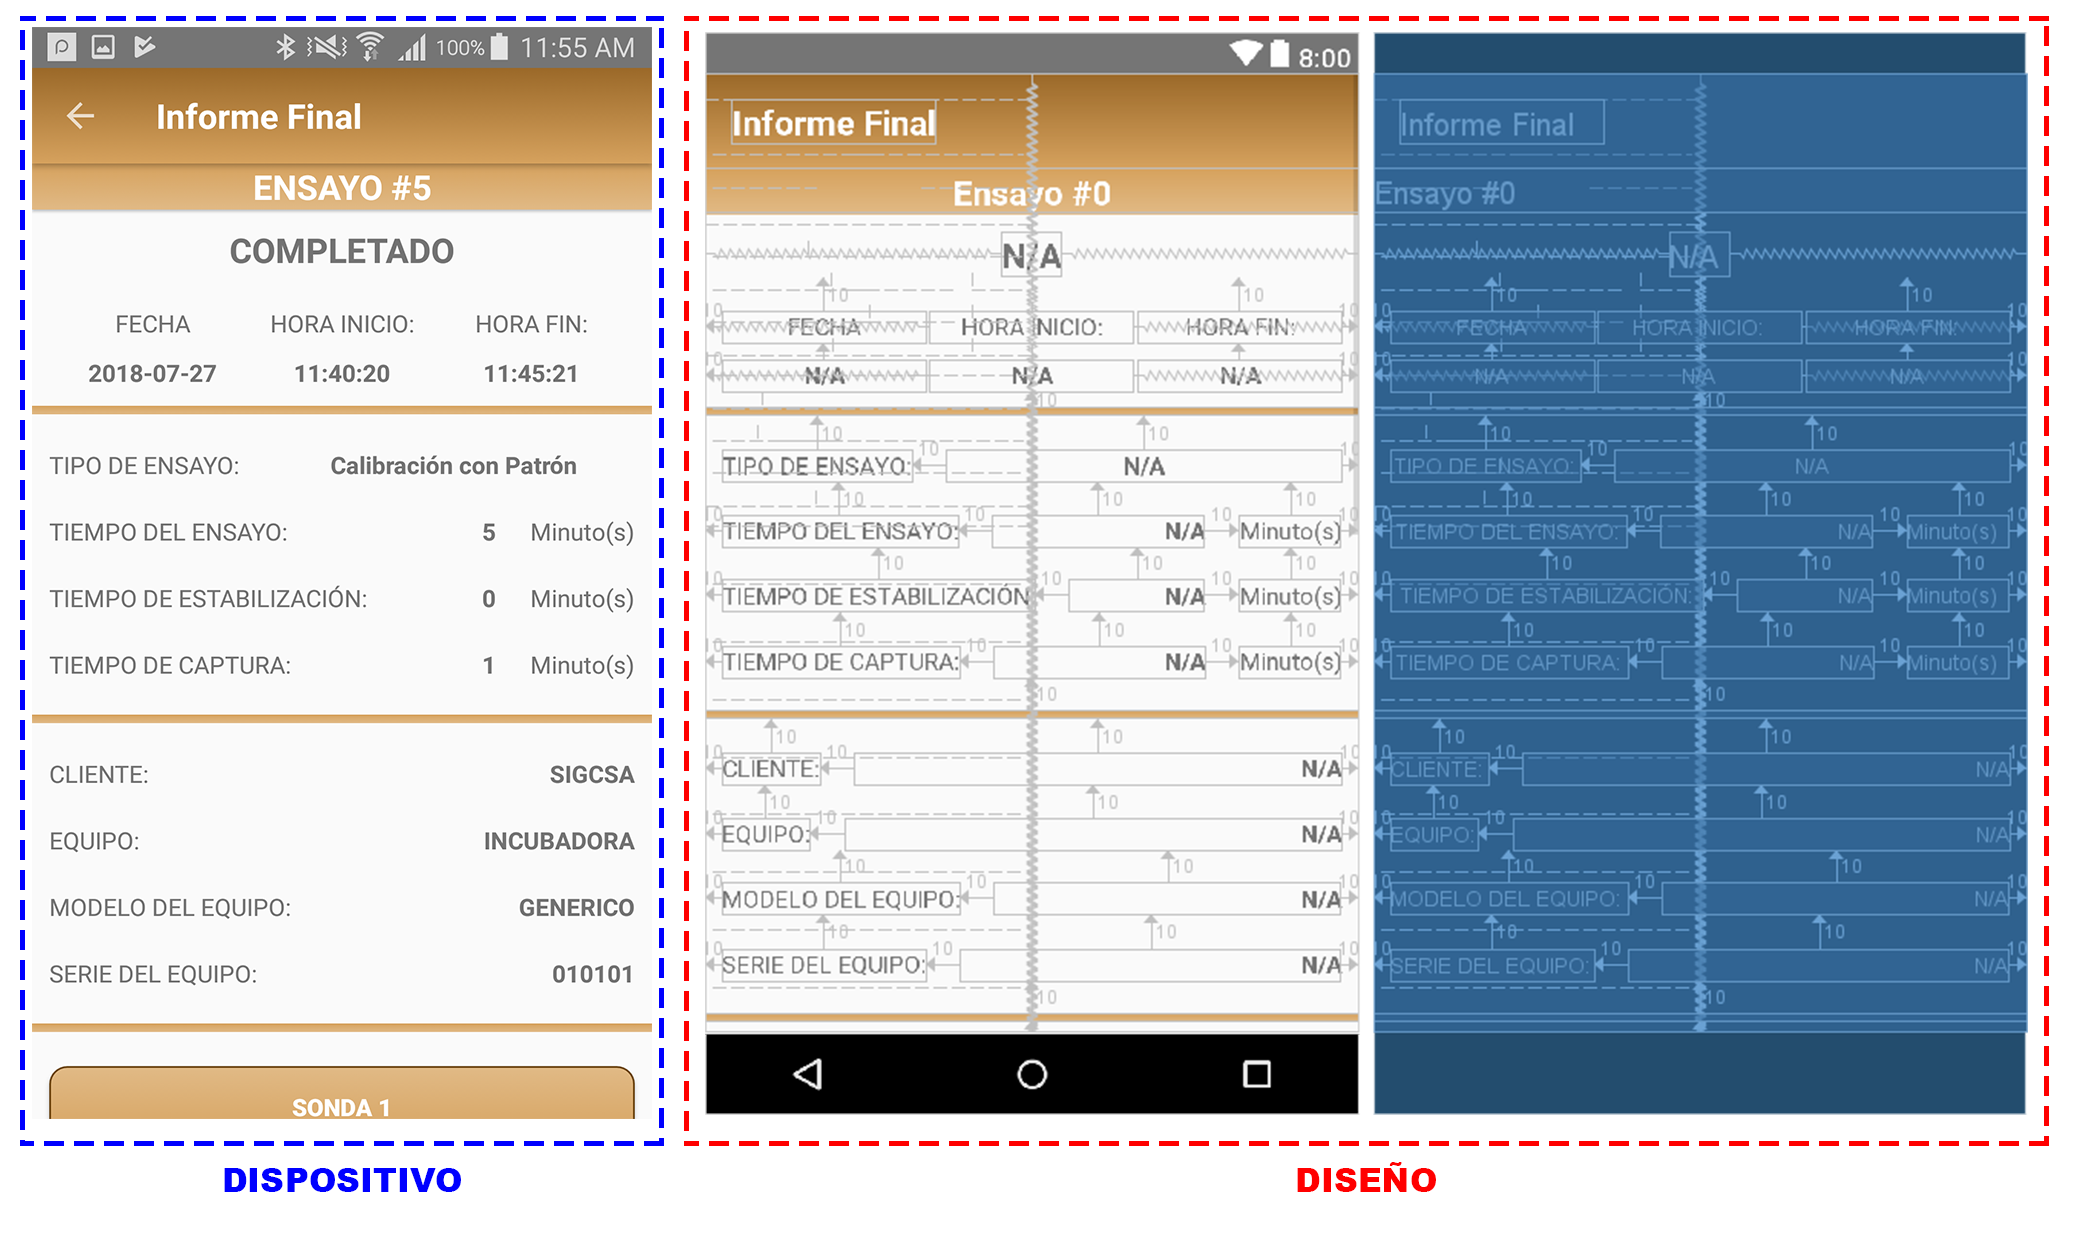
\includegraphics[width=\linewidth]{interfaz11.png}
	\caption{Interfaz y diseño de la actividad detalle}
\end{figure}

\par \noindent
Al inicio de la interfaz de esta actividad se encuentra el "toolbar" o barra de navegación con el texto "Informe Final" y un botón para regresar a la actividad principal. Seguido un texto con un fondo del color de la aplicación con el texto "Ensayo" junto con su respectivo ID en la base de datos. En la primera sección se indica al usuario si el ensayo fue "COMPLETADO" en caso tal que no haber ningún problema durante la captura de la información y en caso contrario que el usuario haya presionado el botón cancelar el texto será "CANCELADO". Luego datos esenciales como la fecha de ejecución del ensayo, hora de inicio del ensayo y hora de finalización del ensayo.

\par \noindent
Luego sigue información de los parámetros seleccionados y escritos por el usuario para el ensayo. Por último se encuentra un botón con el texto "Sonda 1". La cantidad botones dependerá del tipo de ensayo que se ha realizado. De la misma manera como es dinámico el texto del "Estado del Sistema" en el fragmento añadir. Estos botones son especiales ya que al presionarlos se inicia la actividad detalle sonda.

\subsubsection{Actividad Detalle Sonda}

\begin{figure}[H]
	\centering
	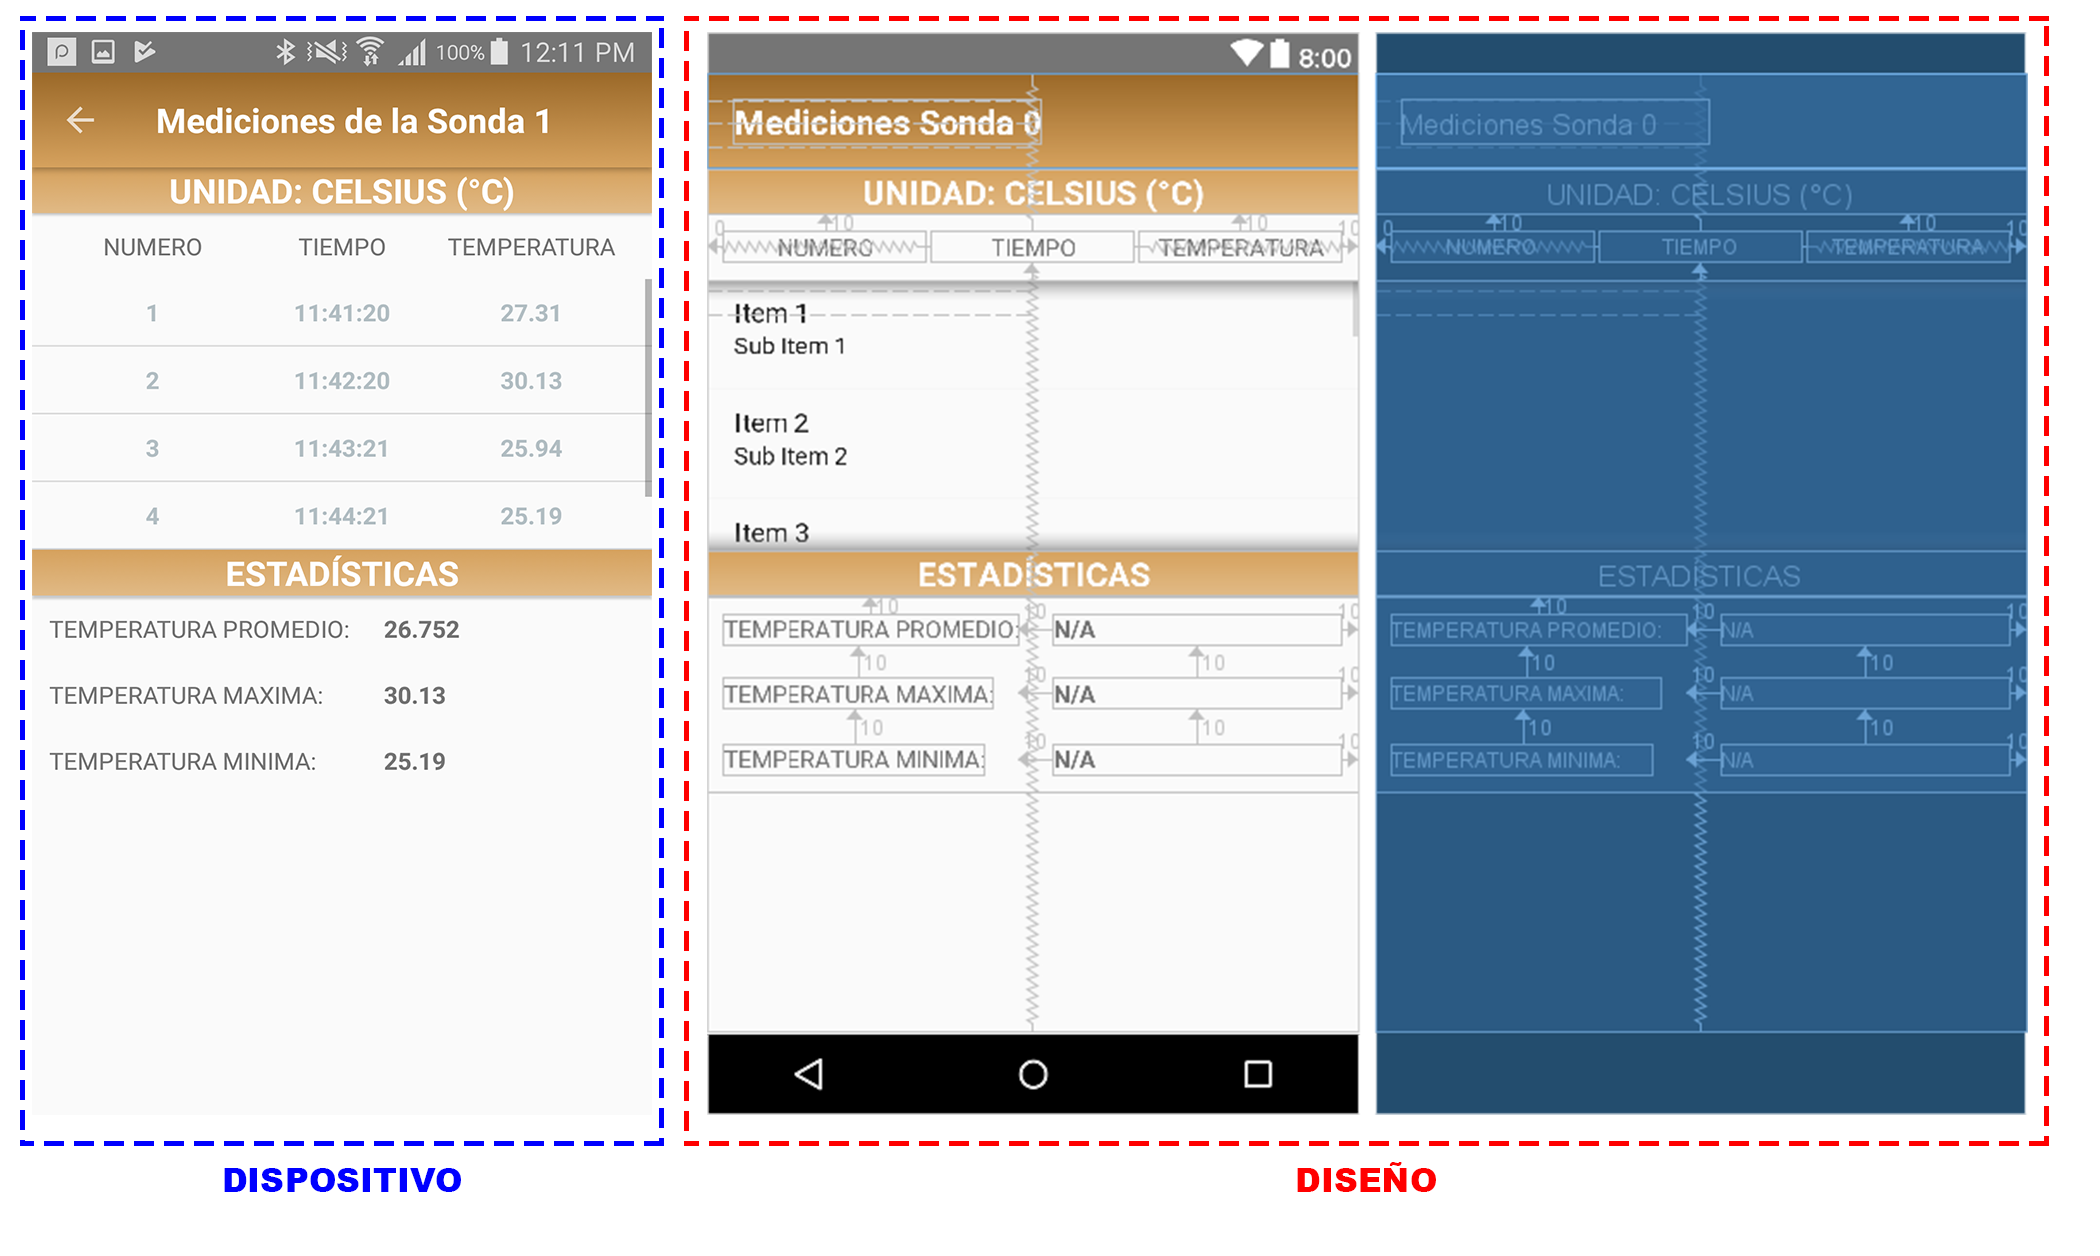
\includegraphics[width=\linewidth]{interfaz12.png}
	\caption{Interfaz y diseño de la actividad detalle}
\end{figure}

\par \noindent
La actividad detalle sonda es donde se muestran las mediciones de temperaturas capturadas por la sonda de un prototipo. Pero ¿Por qué una actividad o una interfaz para cada sonda? recordemos que en Android hay que mantener la aplicación fluida para una buena experiencia del usuario. En el peor de los casos si el usuario selecciona un tipo de caracterización "Isotermos 1" donde se tomará las mediciones de 9 sondas y si se selecciona capturar cada minuto tenemos un total de 60 mediciones por 9 sondas. Esto puede afectar el rendimiento de la aplicación al renderizar esa gran cantidad de texto en menos de 1 segundo.

\par \noindent
Otra de las razones es para mantener mejor organizada la información y una interfaz más amigable. La interfaz de la actividad detalle sonda consta de un "toolbar" con un texto indicando su respectiva sonda y un botón para regresar a la actividad detalle. Seguido de un texto con un fondo del color de la aplicación indicando la escala de temperatura utilizada en el ensayo por la sonda. Seguido de una tabla indicando el número de medida, el tiempo en que se tomó esa medida y la medida de temperatura capturada. La tabla es un "ListView" y es deslizable. Seguido un texto con un fondo de color de aplicación con el texto "ESTADÍSTICAS"; por último se muestran 3 textos indicando valores estadísticos con respecto a la sonda. Valores como promedio de temperatura y valor máximo y mínimo de temperatura.

\par \noindent
Teniendo en cuenta el conocimiento de todas las interfaces y las funciones de sus componentes en ellas es necesario definir como realizar ciertas tareas o funciones de la aplicación.
